\documentclass[10pt,b6paper,usenames,twoside]{article} 
\usepackage[utf8x]{inputenc} 
\usepackage[italian,english,francais]{babel} 
\usepackage{calligra}
\usepackage[T1]{fontenc} 	
%\usepackage{fontspec} 
%\usepackage{xunicode} 
%\usepackage{xltxtra} 
\usepackage{lipsum} 
\usepackage{graphicx}
\usepackage[rightcaption,raggedright]{sidecap}
\usepackage{caption}


%\usepackage[utf8]{inputenc}
%\usepackage[T1]{fontenc}
\usepackage{geometry}
\usepackage{verbatim}
\usepackage{hyperref}
\usepackage[super]{nth}
\usepackage{tikz}
\usepackage{harmony}
%\usepackage{musixtex}
\usepackage{amsmath,amssymb,amsfonts,amsthm}
\usepackage{bm}
\usepackage{epstopdf}
\usepackage{longtable}

%\usepackage[LY1]{fontenc} 
%\renewcommand{\rmdefault}{AJensonPro} 
%\renewcommand{\bfdefault}{b} 

\usepackage{xcolor}
%\definecolor{forestgreen(traditional)}{rgb}{0.0, 0.27, 0.13}
\definecolor{forestgreen(traditional)}{rgb}{0.0, 0.44, 0.0} % Hooker's
%\definecolor{forestgreen(traditional)}{rgb}{0.03, 0.47, 0.19} % La Salle
%\definecolor{forestgreen(traditional)}{rgb}{0.0, 0.35, 0.08} % Nostro!
\definecolor{cream}{rgb}{1.0, 0.99, 0.8}
%\color{forestgreen(traditional)}

%\setmainfont[Mapping=tex-text]{Adobe Jenson Pro} 

\usepackage{bbding} 
\usepackage{microtype} 
%\usepackage[usenames,dvipsnames]{xcolor} 
%\usepackage[bf,sc,rm,tiny,raggedright]{titlesec} 
%\usepackage{oldstyle} 
%\usepackage[small,sc]{titlesec} 
\usepackage{geometry} 
\geometry{centering}  %,nohead
\geometry{width=90mm,height=130mm} 

%\usepackage[noprint]{booklet} 
\usepackage[noprint]{booklet}% 
\nofiles 
\pagespersignature{4} 

%\usepackage{pifont} 

\usepackage{fancyhdr}
\renewcommand{\headrulewidth}{0.0pt}
\pagestyle{fancy}
\fancyhf{}
\fancyhead[LE]{\textcolor{forestgreen(traditional)}{\calligra Giovanni Paolo e \hspace*{-3mm} Clara}}
\fancyhead[RO]{\textcolor{forestgreen(traditional)}{\calligra 5 settembre 2015}}
\fancyfoot[C]{\thepage}

\usepackage{afterpage}
\newcommand\blankpage{%
    \null
    \thispagestyle{empty}%
    \addtocounter{page}{-1}%
    \newpage}

\begin{document} 
\shorthandoff{;:}
%\color{forestgreen(traditional)}
\setpdftargetpages 
% <pagine 1-12> 

\afterpage{\blankpage}

\begin{titlepage}
\color{forestgreen(traditional)}
\begin{center}

%\vspace*{5cm}

\textcalligra{\huge{Giovanni Paolo e \hspace*{-6mm} Clara}}\\
\textcalligra{\Large{5 settembre 2015}}\\

\vspace*{1.5cm}
%\includegraphics[width=10cm,keepaspectratio]{camaldola_print.jpg}
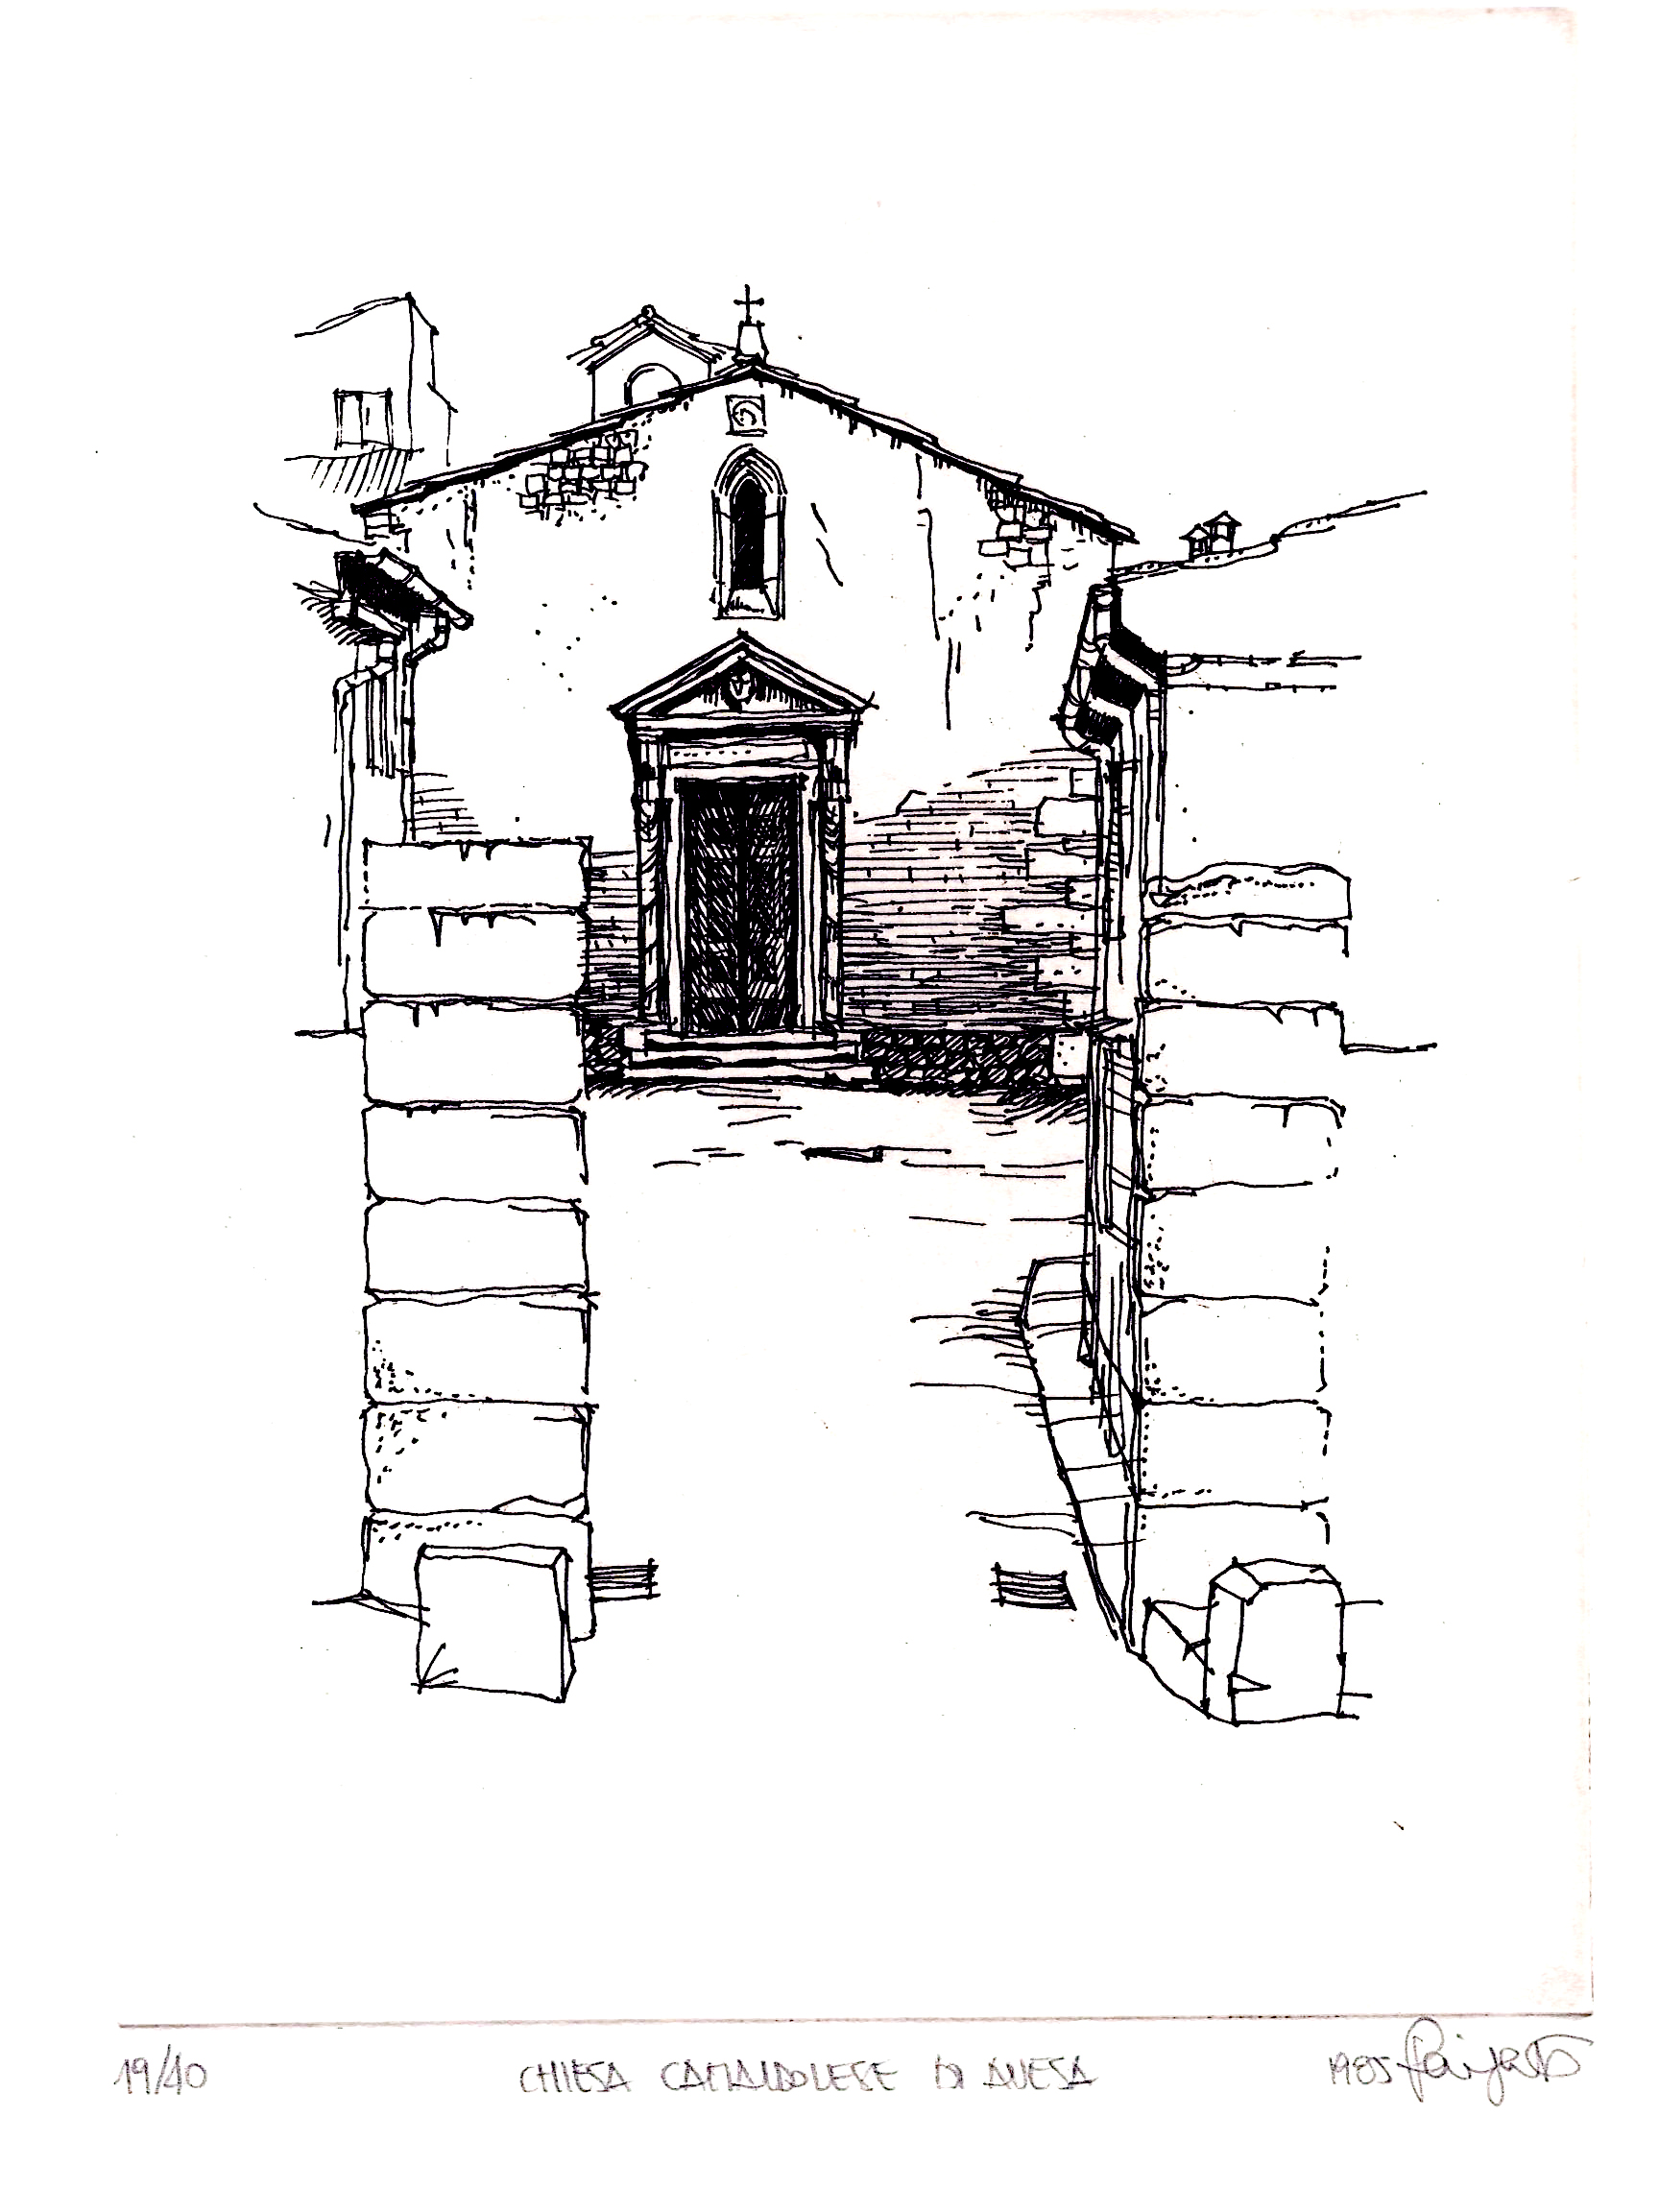
\includegraphics[scale=0.13, trim=80mm 180mm 80mm 100mm, clip=true]{camaldola_print_4.jpg}

\vspace*{1.5cm}

\textcalligra{\Large{
%5 settembre 2015\\
Chiesa di Camaldola\\
Avesa - Verona\\
}}

\end{center}
\color{black}
\end{titlepage}

\afterpage{\blankpage}


\thispagestyle{empty}%
    \addtocounter{page}{-1}%
    \newpage
%\par\vspace*{\fill}

\vspace*{10mm}
\begin{center}
\textcolor{forestgreen(traditional)}{\hspace*{-5mm} \textcalligra{\LARGE{Celebranti}}}\\
\vspace*{3mm}
\normalsize{Don Michele Nicolis\\
Don Giuliano Zanini}

\vspace*{15mm}

\textcolor{forestgreen(traditional)}{\hspace*{-5mm} \textcalligra{\LARGE{Musiche}}}\\
\vspace*{3mm}
\normalsize{Elena Cipriani, mezzosoprano e violino\\
Paolo De Zen, organo\\
Rita Poli, violino\\
Nicola Vignola, fisarmonica}
	
\vspace*{15mm}

%\textcolor{forestgreen(traditional)}{\hspace*{-5mm}\textcalligra{\LARGE{Testimoni}}}\\
\vspace*{0mm}
\normalsize{
\begin{minipage}[t]{0.48\textwidth}
\begin{flushleft}
\textcolor{forestgreen(traditional)}{\hspace*{-0mm}\textcalligra{\LARGE{Testimoni sposo}}}\\
\vspace*{3mm}
Francesco Cottini\\
Lorenzo Di Paola\\
Davide Minardi
\end{flushleft}
\end{minipage}
\hfill
\begin{minipage}[t]{0.48\textwidth}
\begin{flushright}
\textcolor{forestgreen(traditional)}{\hspace*{-5mm}\textcalligra{\LARGE{Testimoni sposa}}}\\
\vspace*{3mm}
Roxanne Loos\\
Nicola Vignola\\
Laura Zampieri\\
\end{flushright}
\end{minipage}
	}

\end{center}

\vspace*{-0cm}

\clearpage

%\color{black}
%\part*{RITO DEL MATRIMONIO} 

\setcounter{page}{1}

\noindent \textcolor{forestgreen(traditional)}{\Acht} \hspace*{0mm} R. Wagner, \textit{Marcia nuziale}

\section*{\textcolor{forestgreen(traditional)}{\textcalligra{\huge{Riti di introduzione}}}} 
\noindent Nel nome del Padre e del Figlio e dello Spirito Santo.\\ \textbf{Amen.} 
\\ 
La grazia del Signore nostro Gesù Cristo, l'amore di Dio Padre e la comunione dello Spirito Santo sia con tutti voi. \textbf{E con il tuo spirito.} 

\subsection*{\textcolor{forestgreen(traditional)}{MEMORIA DEL BATTESIMO}} 
\noindent Fratelli e sorelle, ci siamo riuniti con gioia nella casa del Signore nel giorno in cui \textcolor{forestgreen(traditional)}{\textsc{Giovanni Paolo}} e \textcolor{forestgreen(traditional)}{\textsc{Clara}} intendono formare la loro famiglia. In quest'ora di particolare grazia siamo loro vicini con l'affetto, con l’amicizia e la preghiera fraterna. Ascoltiamo attentamente insieme con loro la Parola che Dio oggi ci rivolge. In unione con la santa Chiesa supplichiamo Dio Padre, per Cristo Signore nostro, perché benedica questi suoi figli che stanno per celebrare il loro Matrimonio, li accolga nel suo amore e li costituisca in unità.

\noindent Facciamo ora memoria del Battesimo, nel quale siamo rinati a vita nuova.
Divenuti figli nel Figlio, riconosciamo con gratitudine il dono ricevuto, per rimanere fedeli all'amore a cui siamo stati chiamati.\\
 
\noindent Padre, nel Battesimo del tuo Figlio Gesù al fiume Giordano hai rivelato al mondo l'amore sponsale per il tuo popolo.\\ 
\textbf{Noi ti lodiamo e ti rendiamo grazie.}\smallskip 
\\ 
Cristo Gesù, dal tuo costato aperto sulla Croce, hai generato la Chiesa, tua diletta sposa.\\ 
\textbf{Noi ti lodiamo e ti rendiamo grazie.}\smallskip 
\\ 
Spirito Santo, potenza del Padre e del Figlio, oggi fai risplendere in \textcolor{forestgreen(traditional)}{\textsc{Giovanni Paolo}} e \textcolor{forestgreen(traditional)}{\textsc{Clara}} la veste nuziale della Chiesa.\\ 
\textbf{Noi ti lodiamo e ti rendiamo grazie.}\\

\noindent Dio onnipotente, origine e fonte della vita, che ci hai rigenerati nell'acqua con la potenza del tuo Spirito, ravviva in tutti noi la grazia del Battesimo, e concedi a \textcolor{forestgreen(traditional)}{\textsc{Giovanni Paolo}} e \textcolor{forestgreen(traditional)}{\textsc{Clara}} un cuore libero e una fede ardente perché, purificati nell'intimo, accolgano il dono del Matrimonio, nuova via della loro santificazione. Per Cristo nostro Signore.\\ \textbf{Amen.} 

\subsection*{\textcolor{forestgreen(traditional)}{INNO DI LODE}}

\noindent \textcolor{forestgreen(traditional)}{\Acht}\hspace*{0mm} \textit{Glory to God in the highest}
\\ 


\hfill\begin{minipage}{\dimexpr\textwidth-1cm}
\textbf{\textit{Glory to God in the highest,\\
Glory to God in the highest,\\
Glory to God, Glory to God\\
And on earth peace to people of good will.}}\\
\end{minipage}

\noindent \textit{We praise you, we bless you,\\
We adore you, we glorify you,\\
We give you thanks for your great glory,\\
Lord God, heavenly King, O God, almighty Father.}\\

\hfill\begin{minipage}{\dimexpr\textwidth-1cm}
\textbf{\textit{Glory to God in the highest $\hdots$}}\\
\end{minipage}

\noindent \textit{Lord Jesus Christ, only Begotten Son,\\
Lord God, Lamb of God, Son of the Father.\\
You take away the sins of the world,\\
Have mercy on us.\\
You take away the sins of the world,\\ 
Receive our prayer\\
You are seated at the right hand of the Father,\\
Have mercy on us.}\\

\hfill\begin{minipage}{\dimexpr\textwidth-1cm}
\textbf{\textit{Glory to God in the highest $\hdots$}}\\
\end{minipage}

\noindent \textit{For you alone are the Holy One,\\
You alone are the Lord,\\
You alone are the Most High Jesus Christ,\\
With the Holy Spirit, in the glory of God the Father.\\ 
Amen.}\\

\hfill\begin{minipage}{\dimexpr\textwidth-1cm}
\textbf{\textit{Glory to God in the highest $\hdots$}}\\
\end{minipage}

\subsection*{\textcolor{forestgreen(traditional)}{COLLETTA}} 
\noindent Ascolta, Signore, la nostra preghiera ed effondi con bontà la tua grazia su \textcolor{forestgreen(traditional)}{\textsc{Giovanni Paolo}} e \textcolor{forestgreen(traditional)}{\textsc{Clara}}, perché, unendosi davanti al tuo altare, siano confermati nel reciproco amore. Per il nostro Signore Gesù Cristo, tuo Figlio, che è Dio, e vive e regna con te, nell'unità dello Spirito Santo, per tutti i secoli dei secoli.\\ \textbf{Amen.} 
\clearpage

\section*{\textcolor{forestgreen(traditional)}{\textcalligra{\huge{Liturgia della Parola}}}}
\noindent Fratelli e sorelle, dopo aver fatto memoria del Battesimo, ascoltiamo in raccoglimento la parola di Dio. Accolta con fede, annuncia la presenza del Signore in questo momento di festa e di gioia, illumina il cammino dei coniugi, apre alla ricchezza della vita ecclesiale, rivela l'amore di Cristo sposo per la Chiesa sua sposa.
 
\subsection*{\textcolor{forestgreen(traditional)}{PRIMA LETTURA}} 
\noindent \textbf{Dal libro del profeta Ezechiele} \hfill \textcolor{forestgreen(traditional)}{\textit{36,24--28}}\\ 
\textcolor{forestgreen(traditional)}{\textit{\footnotesize{Porrò il mio spirito dentro di voi.}}}\\ 

Vi prenderò dalle genti, dice il Signore, vi radunerò da ogni terra e vi condurrò sul vostro suolo. Vi aspergerò con acqua pura e sarete purificati; io vi purificherò da tutte le vostre impurità e da tutti i vostri idoli; vi darò un cuore nuovo, metterò dentro di voi uno spirito nuovo, toglierò da voi il cuore di pietra e vi darò un cuore di carne.

Porrò il mio spirito dentro di voi e vi farò vivere secondo i miei statuti e vi farò osservare e mettere in pratica le mie leggi. Abiterete nella terra che io diedi ai vostri padri; voi sarete il mio popolo e io sarò il vostro Dio.

\noindent Parola di Dio.\\ \textbf{Rendiamo grazie a Dio.}

\clearpage
 
\subsection*{\textcolor{forestgreen(traditional)}{FIRST READING}} 
\noindent \textbf{A reading from the Book of the prophet Eze- \linebreak kiel}\hfill \textcolor{forestgreen(traditional)}{\textit{36,24--28}} \\ 
\textcolor{forestgreen(traditional)}{\textit{\footnotesize{I will put My Spirit within you.}}} \\ 

For I will take you from among the nations, gather you out of all countries, and bring you into your own land. Then I will sprinkle clean water on you, and you shall be clean; I will cleanse you from all your filthiness and from all your idols. I will give you a new heart and put a new spirit within you; I will take the heart of stone out of your flesh and give you a heart of flesh. 

I will put My Spirit within you and cause you to walk in My statutes, and you will keep My judgments and do them. Then you shall dwell in the land that I gave to your fathers; you shall be My people, and I will be your God.

\noindent The Word of the Lord.\\ \textbf{Thanks be to God.}

\subsection*{\textcolor{forestgreen(traditional)}{\textsc{SALMO RESPONSORIALE}}} 

\noindent \textcolor{forestgreen(traditional)}{\Acht}\hspace*{0mm} \textit{dal Salmo 111}
\\ 
%\textbf{Beato chi cammina nella legge del Signore.}\\

\hfill\begin{minipage}{\dimexpr\textwidth-1cm}
\textbf{\textit{Beato chi cammina nella legge del Signore.}}\\
\end{minipage}

\noindent \textit{Beato l'uomo che teme il Signore\\ 
e trova grande gioia nei suoi comandamenti.\\ 
Potente sulla terra sarà la sua stirpe,\\ 
la discendenza dei giusti sarà benedetta.}\\ 

\hfill\begin{minipage}{\dimexpr\textwidth-1cm}
\textbf{\textit{Beato chi cammina nella legge del Signore.}}\\
\end{minipage}

\noindent \textit{Onore e ricchezza nella sua casa,\\
la sua giustizia rimane per sempre.\\
Spunta nelle tenebre come luce per i giusti,\\
buono, misericordioso e giusto.}\\

\hfill\begin{minipage}{\dimexpr\textwidth-1cm}
\textbf{\textit{Beato chi cammina nella legge del Signore.}}\\
\end{minipage}

\noindent \textit{Felice l'uomo pietoso che da in prestito,\\
amministra i suoi beni con giustizia.\\
Non temerà annunzio di sventura.}\\

\hfill\begin{minipage}{\dimexpr\textwidth-1cm}
\textbf{\textit{Beato chi cammina nella legge del Signore.}}\\
\end{minipage}

\noindent \textit{Saldo è il suo cuore, confida nel Signore.\\
Sicuro è il suo cuore, non teme,\\
finché trionferà dei suoi nemici.}\\

\hfill\begin{minipage}{\dimexpr\textwidth-1cm}
\textbf{\textit{Beato chi cammina nella legge del Signore.}}\\
\end{minipage}

\noindent \textit{Egli dona largamente ai poveri,\\
la sua giustizia rimane per sempre,\\
la sua potenza s'innalza nella gloria.}\\

\hfill\begin{minipage}{\dimexpr\textwidth-1cm}
\textbf{\textit{Beato chi cammina nella legge del Signore.}}\\
\end{minipage}

\subsection*{\textcolor{forestgreen(traditional)}{SECONDA LETTURA}} 
\noindent \textbf{Dalla lettera di san Paolo apostolo ai Ro- \linebreak mani} \hfill \textcolor{forestgreen(traditional)}{\textit{12,1--2.9--18}}\\ 
\textcolor{forestgreen(traditional)}{\textit{\footnotesize{Offrite i vostri corpi come sacrificio vivente, santo e gradito a Dio.}}}\\ 

Vi esorto dunque, fratelli, per la misericordia di Dio, a offrire i vostri corpi come sacrificio vivente, santo e gradito a Dio; è questo il vostro culto spirituale. Non conformatevi a questo mondo, ma lasciatevi trasformare rinnovando il vostro modo di pensare, per poter discernere la volontà di Dio, ciò che è buono, a lui gradito e perfetto. 

La carità non sia ipocrita: detestate il male, attaccatevi al bene; amatevi gli uni gli altri con affetto fraterno, gareggiate nello stimarvi a vicenda. Non siate pigri nel fare il bene, siate invece ferventi nello spirito; servite il Signore. Siate lieti nella speranza, costanti nella tribolazione, perseveranti nella preghiera. Condividete le necessità dei santi; siate premurosi nell'ospitalità.

% cos\`i  % NOTE ACCENT 
Benedite coloro che vi perseguitano, benedite e non maledite. Rallegratevi con quelli che sono nella gioia; piangete con quelli che sono nel pianto. Abbiate i medesimi sentimenti gli uni verso gli altri; non nutrite desideri di grandezza; volgetevi piuttosto a ciò che è umile. Non stimatevi sapienti da voi stessi. 
  
Non rendete a nessuno male per male. Cercate di compiere il bene davanti a tutti gli uomini. Se possibile, per quanto dipende da voi, vivete in pace con tutti. 

\noindent Parola di Dio.\\ \textbf{Rendiamo grazie a Dio.}
 
\subsection*{\textcolor{forestgreen(traditional)}{SECOND READING}} 
\noindent \textbf{A reading from the Letter of Saint Paul to the Romans} \hfill \textcolor{forestgreen(traditional)}{\textit{12,1--2.9--18}}\\ 
\textcolor{forestgreen(traditional)}{\textit{\footnotesize{Offering your living bodies as a holy sacrifice, truly pleasing to God.}}}\\ 

Think of God's mercy, my brothers, and worship him, I beg you, in a way that is worthy of thinking beings, by offering your living bodies as a holy sacrifice, truly pleasing to God. Do not model yourselves on the behaviour of the world around you, but let your behaviour change, modelled by your new mind. This is the only way to discover the will of God and know what is good, what it is that God wants, what is the perfect thing to do. 

Do not let your love be a pretence, but sincerely prefer good to evil. Love each other as much as brothers should, and have a profound respect for each other. Work for the Lord with untiring effort and with great earnestness of spirit. If you have hope, this will make you cheerful. Do not give up if trials come; and keep on praying. If any of the saints are in need you must share with them; and you should make hospitality your special care.

% cos\`i  % NOTE ACCENT 
Bless those who persecute you: never curse them, bless them. Rejoice with those who rejoice and be sad with those in sorrow. Treat everyone with equal kindness; never be condescending but make real friends with the poor. Do not allow yourself to become self-satisfied. Never repay evil with evil but let everyone see that you are interested only in the highest ideals. Do all you can to live at peace with everyone.  

\noindent The Word of the Lord.\\ \textbf{Thanks be to God.}\\


\noindent \textcolor{forestgreen(traditional)}{\Acht} \hspace*{0mm} W. A. Mozart, \textit{Alleluja (Exsultate, jubilate)} \\ 

\noindent \textbf{Alleluia, alleluia.}\\
\vspace*{-0.5mm}
\hfill\begin{minipage}{\dimexpr\textwidth-1cm}
\vspace*{1mm}\textit{Invita alla tua cena chiunque ha bisogno;\\
Dio stesso sarà la tua ricompensa.
}
\end{minipage} 

\noindent \textbf{Alleluia.}
\subsection*{\textcolor{forestgreen(traditional)}{VANGELO}} 

\noindent \textcolor{forestgreen(traditional)}{\CrossMaltese} \ \textbf{Dal Vangelo secondo Giovanni} \hfill \textcolor{forestgreen(traditional)}{\textit{2,1--11}}\\ 
\textcolor{forestgreen(traditional)}{\textit{\footnotesize{Così Gesù diede inizio ai suoi miracoli in Cana di Galilea.}}} \\ 

In quel tempo, ci fu uno sposalizio a Cana di Galilea e c’era la madre di Gesù. Fu invitato alle nozze anche Gesù con i suoi discepoli. Nel frattempo, venuto a mancare il vino, la madre di Gesù gli disse: «Non hanno più vino». E Gesù rispose: «Che ho da fare con te, o donna? Non è ancora giunta la mia ora». La madre dice ai servi: «Fate quello che vi dirà».

Vi erano là sei giare di pietra per la purificazione dei Giudei, contenenti ciascuna due o tre barili. E Gesù disse loro: «Riempite d’acqua le giare»; e le riempirono fino all’orlo. Disse loro di nuovo: «Ora attingete e portatene al maestro di tavola». Ed essi gliene portarono. E come ebbe assaggiato l’acqua diventata vino, il maestro di tavola, che non sapeva di dove venisse (ma lo sapevano i servi che avevano attinto l’acqua), chiamò lo sposo e gli disse: «Tutti servono da principio il vino buono e, quando sono un po’ brilli, quello meno buono; tu invece hai conservato fino ad ora il vino buono». Così Gesù diede inizio ai suoi miracoli in Cana di Galilea, manifestò la sua gloria e i suoi discepoli credettero in lui. 

\noindent Parola del Signore.\\ \textbf{Lode a te, o Cristo.}\\
\clearpage

\subsection*{\textcolor{forestgreen(traditional)}{GOSPEL}} 


\noindent \textcolor{forestgreen(traditional)}{\CrossMaltese} \hspace*{1mm} \textbf{A reading from the Gospel according to\linebreak John} \hfill \textcolor{forestgreen(traditional)}{\textit{2,1--11}}\\ 
\textcolor{forestgreen(traditional)}{\textit{\footnotesize{This was the first of the signs given by Jesus at Cana in Galilee.}}} \\ 
%: it was given

There was a wedding at Cana in Galilee. The mother of Jesus was there, and Jesus and his disciples had also been invited. When they ran out of wine, since the wine provided for the wedding was all finished, the mother of Jesus said to him, «They have no wine». Jesus said, «Woman why turn to me? My hour has not come yet». His mother said to the servants, «Do whatever he tells you». 

There were six stone water jars standing there, meant for the ablutions that are customary among the Jews: each could hold twenty or thirty gallons. Jesus said to the servants, «Fill the jars with water», and they filled them to the brim. «Draw some out now», he told them, «and take it to the steward». They did this; the steward tasted the water, and it had turned into wine. Having no idea where it came from - only the servants who had drawn the water knew - the steward called the bridegroom and said, «People generally serve the best wine first, and keep the cheaper sort till the guests have had plenty to drink, but you have kept the best wine till now».
This was the first of the signs given by Jesus: it was given at Cana in Galilee. He let his glory be seen, and his disciples believed in him.

\noindent The Gospel of the Lord.\\ \textbf{Praise to you, Lord Jesus Christ.}

\clearpage

\section*{\textcolor{forestgreen(traditional)}{\textcalligra{\huge{Liturgia del Matrimonio}}}} 
\subsection*{\textcolor{forestgreen(traditional)}{INTERROGAZIONI PRIMA DEL CON- \linebreak SENSO}} 
\noindent Carissimi \textcolor{forestgreen(traditional)}{\textsc{Giovanni Paolo}} e \textcolor{forestgreen(traditional)}{\textsc{Clara}}, siete venuti insieme nella casa del Padre, perché la vostra decisione di unirvi in Matrimonio riceva il suo sigillo e la sua consacrazione, davanti al ministro della Chiesa e davanti alla comunità. 
\noindent Voi siete già consacrati mediante il Battesimo: ora Cristo vi benedice e vi rafforza con il sacramento nuziale, perché vi amiate l’un l'altro con amore fedele e inesauribile e assumiate responsabilmente i doveri del Matrimonio.
\noindent Pertanto vi chiedo di esprimere davanti alla Chiesa le vostre intenzioni.\\

\noindent \textcolor{forestgreen(traditional)}{\textsc{Giovanni Paolo}} e \textcolor{forestgreen(traditional)}{\textsc{Clara}}, siete venuti a celebrare il Matrimonio senza alcuna costrizione, in piena libertà e consapevoli del significato della vostra decisione?\\ 
\textbf{Sì.}\\ 

\noindent Siete disposti, seguendo la via del Matrimonio, ad amarvi e a onorarvi l'un l'altro per tutta la vita?\\ 
\textbf{Sì.}\\ 

\noindent Siete disposti ad accogliere con amore i figli che Dio vorrà donarvi e a educarli secondo la legge di Cristo e della sua Chiesa?\\ 
\textbf{Sì.} 

\clearpage

\subsection*{\textcolor{forestgreen(traditional)}{MANIFESTAZIONE DEL CONSENSO}} 

\noindent Alla presenza di Dio e davanti alla Chiesa qui riunita, datevi la mano destra ed esprimete il vostro consenso. Il Signore, inizio e compimento del vostro amore, sia con voi sempre.\smallskip 
\\ 

\begin{large} 
\noindent \textbf{Io \textcolor{forestgreen(traditional)}{\textsc{Giovanni Paolo}},\\
accolgo te, \textcolor{forestgreen(traditional)}{\textsc{Clara}}, come mia sposa.\\ 
Con la grazia di Cristo\\ 
prometto di esserti fedele sempre,\\ 
nella gioia e nel dolore,\\ 
nella salute e nella malattia,\\ 
e di amarti e onorarti\\ 
tutti i giorni della mia vita.} 
\end{large}\smallskip 
\\ 
 
\begin{large} 
\noindent \textbf{Io \textcolor{forestgreen(traditional)}{\textsc{Clara}},\\
accolgo te, \textcolor{forestgreen(traditional)}{\textsc{Giovanni Paolo}}, come mio sposo.\\ 
Con la grazia di Cristo\\ 
prometto di esserti fedele sempre,\\ 
nella gioia e nel dolore,\\ 
nella salute e nella malattia,\\ 
e di amarti e onorarti\\ 
tutti i giorni della mia vita.} 
\end{large} 

\subsection*{\textcolor{forestgreen(traditional)}{ACCOGLIENZA DEL CONSENSO}} 

\noindent Il Signore onnipotente e misericordioso confermi il consenso che avete manifestato davanti alla Chiesa e vi ricolmi della sua benedizione.
L’uomo non osi separare ciò che Dio unisce.\\ 
\textbf{Amen.} 

\subsection*{\textcolor{forestgreen(traditional)}{BENEDIZIONE E CONSEGNA DEGLI\linebreak ANELLI}} 

\noindent Signore, benedici \textcolor{forestgreen(traditional)}{\CrossMaltese}\ questi anelli nuziali: gli sposi che li porteranno custodiscano integra la loro fedeltà, rimangano nella tua volontà e nella tua pace e vivano sempre nel reciproco amore. Per Cristo nostro Signore.\\ 
\textbf{Amen.}\\ 

\begin{large} 
\noindent \textbf{\textcolor{forestgreen(traditional)}{\textsc{Clara}}, ricevi questo anello,\\ 
segno del mio amore e della mia fedeltà.\\ 
Nel nome del Padre e del Figlio\\ 
e dello Spirito Santo.} 
\end{large}\\ 

\begin{large} 
\noindent \textbf{\textcolor{forestgreen(traditional)}{\textsc{Giovanni Paolo}}, ricevi questo anello,\\ 
segno del mio amore e della mia fedeltà.\\ 
Nel nome del Padre e del Figlio\\ 
e dello Spirito Santo.} 
\end{large} 

\subsection*{\textcolor{forestgreen(traditional)}{PREGHIERA DEI FEDELI}} 
\noindent Fratelli e sorelle, consapevoli del singolare dono di grazia e carità, per mezzo del quale Dio ha voluto rendere perfetto e consacrare l'amore dei nostri fratelli \textcolor{forestgreen(traditional)}{\textsc{Giovanni Paolo}} e \textcolor{forestgreen(traditional)}{\textsc{Clara}}, chiediamo al Signore che, sostenuti dall'esempio e dall'intercessione dei santi, essi custodiscano nella fedeltà il loro vincolo coniugale.\\ 

\noindent Preghiamo insieme e diciamo:\\ 
\textbf{Dio che sei amore, ascoltaci.}\\


\noindent --- Per \textcolor{forestgreen(traditional)}{\textsc{Giovanni Paolo}} e \textcolor{forestgreen(traditional)}{\textsc{Clara}}, perché il Signore li accompagni sempre lungo il cammino che insieme si apprestano a percorrere, preghiamo.\\ 
\textbf{Dio che sei amore, ascoltaci.}\\ 

\noindent --- For all friends who every day experience the beauty of communion and rejoice in their neighbours' love and happiness. May they continue to build and maintain sincere relationships and mutual trust throughout their entire lifetime. Lord, in your mercy,\\ 
\textbf{Dio che sei amore, ascoltaci.}\\ 

\noindent --- Perché \textcolor{forestgreen(traditional)}{\textsc{Giovanni Paolo}} e \textcolor{forestgreen(traditional)}{\textsc{Clara}}, attraverso l’unione santa del Matrimonio, possano godere della salute del corpo e della salvezza eterna, preghiamo.\\ 
\textbf{Dio che sei amore, ascoltaci.}\\ 

\noindent --- Per tutti i genitori e i parenti, perché abbiano la forza di trasmettere ogni giorno ai propri cari i valori fondanti della famiglia e sappiano essere con i loro comportamenti esempio di vita, preghiamo.\\ 
\textbf{Dio che sei amore, ascoltaci.}\\ 

\noindent --- Pour \textcolor{forestgreen(traditional)}{\textsc{Giovanni Paolo}} et \textcolor{forestgreen(traditional)}{\textsc{Clara}}, qu'ils soient heureux ensemble, que toute difficulté les stimule, que toute joie partagée les rapproche, que leur nouveau couple soit un lien vivant entre les deux familles. Seigneur, nous te prions.\\ 
\textbf{Dio che sei amore, ascoltaci.}\\

\noindent --- Perché il Signore benedica l’unione di \textcolor{forestgreen(traditional)}{\textsc{Giovanni Paolo}} e \textcolor{forestgreen(traditional)}{\textsc{Clara}} come santificò le nozze a Cana di Galilea, preghiamo.\\ 
\textbf{Dio che sei amore, ascoltaci.}\\ 

\noindent --- Per Rita e per i nonni Lidia, Mauro, Fulvia, Ruggero e Mario, che oggi condividono con noi questa immensa gioia dal cielo, dove vivono in pienezza la luce di Dio. Perché accompagnino il cammino di questa nuova famiglia che oggi si forma, preghiamo.\\ 
\textbf{Dio che sei amore, ascoltaci.}\\ 

\noindent --- Perché lo Spirito Santo rinnovi in tutti gli sposi qui presenti la grazia del sacramento del Matrimonio, preghiamo.\\ 
\textbf{Dio che sei amore, ascoltaci.}\\ 

\noindent Ora, in comunione con la Chiesa del cielo, invochiamo l'intercessione dei santi.\\ 

\noindent Santa Maria, Madre di Dio\hfill\textbf{Prega per noi.} \\ 
Santa Maria, Madre della Chiesa\hfill\textbf{Prega per noi.} \\ 
Santa Maria, Regina della famiglia\hfill\textbf{Prega per noi.} \\ 
San Giuseppe, Sposo di Maria\hfill\textbf{Prega per noi.} \\ 
Santi Angeli di Dio\hfill\textbf{Pregate per noi.} \\ 
San Giovanni Battista\hfill\textbf{Prega per noi.} \\ 
Santi Pietro e Paolo\hfill\textbf{Pregate per noi.} \\ 
Sant'Andrea\hfill\textbf{Prega per noi.} \\ 
San Cristoforo\hfill\textbf{Prega per noi.} \\ 
Santa Teresa d’Avila\hfill\textbf{Prega per noi.} \\ 
San Vigilio\hfill\textbf{Prega per noi.} \\ 
Santa Caterina d’Alessandria\hfill\textbf{Prega per noi.} \\ 
San Giorgio\hfill\textbf{Prega per noi.} \\ 
Santa Gudula di Bruxelles\hfill\textbf{Prega per noi.} \\ 
San Domenico Savio \hfill\textbf{Prega per noi.} \\
Santa Francesca Romana\hfill\textbf{Prega per noi.} \\ 
Santi Angeli Custodi\hfill\textbf{Pregate per noi.} \\ 
San Tommaso d’Aquino\hfill\textbf{Prega per noi.} \\ 
Sant’Agostino\hfill\textbf{Prega per noi.} \\ 
San Biagio\hfill\textbf{Prega per noi.} \\ 
San Pio da Pitrelcina\hfill\textbf{Prega per noi.} \\ 
Santa Lidia\hfill\textbf{Prega per noi.} \\ 
Santa Rita\hfill\textbf{Prega per noi.} \\ 
Santa Chiara\hfill\textbf{Prega per noi.} \\ 
San Giovanni Paolo II\hfill\textbf{Prega per noi.} \\ 
San Martino\hfill\textbf{Prega per noi.} \\ 
San Zeno\hfill\textbf{Prega per noi.} \\ 
San Francesco\hfill\textbf{Prega per noi.} \\ 
Santi e Sante tutti di Dio\hfill\textbf{Pregate per noi.} \\ 

\noindent Effondi, Signore, su \textcolor{forestgreen(traditional)}{\textsc{Giovanni Paolo}} e \textcolor{forestgreen(traditional)}{\textsc{Clara}} lo Spirito del tuo amore, perché diventino un cuore solo e un'anima sola: nulla separi questi sposi che tu hai unito, e, ricolmati della tua benedizione, nulla li affligga. Per Cristo nostro Signore.\\ 
\textbf{Amen.} 

\clearpage

\section*{\textcolor{forestgreen(traditional)}{\textcalligra{\huge{Liturgia Eucaristica}}}} 
\vspace*{-1mm}
\noindent \textcolor{forestgreen(traditional)}{\Acht} \hspace*{0mm}  \textit {Su ali d'aquila}\\
%\vspace*{1mm}

\noindent \textit{Tu che abiti al riparo del Signore\\
e che dimori alla Sua ombra\\
dì al Signore «Mio rifugio,\\
mia roccia in cui confido».}\\

\hfill\begin{minipage}{\dimexpr\textwidth-1cm}
\textbf{\textit{E ti rialzerà, ti solleverà\\
su ali d'aquila ti reggerà\\
sulla brezza dell'alba ti farà brillar\\
come il sole, così nelle Sue mani vivrai.}}\\
\end{minipage}

\noindent \textit{Dal laccio del cacciatore ti libererà\\
e dalla carestia che distrugge.\\
Poi ti coprirà con le sue ali\\
e rifugio troverai.}\\

\hfill\begin{minipage}{\dimexpr\textwidth-1cm}
\textbf{\textit{E ti rialzerà, ti solleverà $\hdots$}}\\
\end{minipage}

\noindent \textit{Non devi temere i terrori della notte\\
né freccia che vola di giorno\\
mille cadranno al tuo fianco\\
ma nulla ti colpirà.}\\

\hfill\begin{minipage}{\dimexpr\textwidth-1cm}
\textbf{\textit{E ti rialzerà, ti solleverà $\hdots$}}\\
\end{minipage}

\noindent \textit{Perché ai suoi angeli ha dato un comando\\
di preservarti in tutte le tue vie\\
ti porteranno sulle loro mani\\
contro la pietra non inciamperai.}
\clearpage

\hfill\begin{minipage}{\dimexpr\textwidth-1cm}
\textbf{\textit{E ti rialzerà, ti solleverà $\hdots$}}\\
\end{minipage}

\hfill\begin{minipage}{\dimexpr\textwidth-1cm}
\textbf{\textit{E ti rialzerò, ti solleverò\\
su ali d'aquila ti reggerò\\
sulla brezza dell'alba ti farò brillar\\
come il sole,\\
così nelle Mie mani vivrai.}}\\
\end{minipage}


\subsection*{\textcolor{forestgreen(traditional)}{ORAZIONE SULLE OFFERTE}} 
\noindent O Dio, Padre di bontà, accogli il pane e il vino, che la tua famiglia ti offre con intima gioia, e custodisci nel tuo amore \textcolor{forestgreen(traditional)}{\textsc{Giovanni Paolo}} e \textcolor{forestgreen(traditional)}{\textsc{Clara}} che hai unito con il sacramento nuziale. Per Cristo nostro Signore.\\ 
\textbf{Amen.} 
\subsection*{\textcolor{forestgreen(traditional)}{PREFAZIO}} 
\noindent Il Signore sia con voi.\\ 
\textbf{E con il tuo spirito.}\smallskip 
\\ 
In alto i nostri cuori.\\ 
\textbf{Sono rivolti al Signore.}\smallskip 
\\ 
Rendiamo grazie al Signore, nostro Dio.\\ 
\textbf{\`{E} cosa buona e giusta.}\\ 

\noindent \`{E} veramente cosa buona e giusta, nostro dovere e fonte di salvezza, rendere grazie sempre e in ogni luogo a te, Signore, Padre santo, Dio onnipotente ed eterno. 
\clearpage
\noindent Tu hai dato alla comunità coniugale la dolce legge dell'amore e il vincolo indissolubile della pace, perché l'unione casta e feconda degli sposi accresca il numero dei tuoi figli. 

\noindent Con disegno mirabile hai disposto che la nascita di nuove creature allieti l'umana famiglia, e la loro rinascita in Cristo edifichi la tua Chiesa. 

\noindent Per questo mistero di salvezza, uniti agli angeli e ai santi, invochiamo insieme l'inno della tua gloria:\\ 

\noindent \textbf{Santo, Santo, Santo il Signore Dio dell'universo.\\ I cieli e la terra sono pieni della tua gloria.\\ Osanna nell'alto dei cieli.\\ Benedetto colui che viene nel nome del Signore.\\ Osanna nell'alto dei cieli.} 

\subsection*{\textcolor{forestgreen(traditional)}{PREGHIERA EUCARISTICA}} 

\noindent \textcolor{forestgreen(traditional)}{\textit{\footnotesize{Il celebrante recita la Preghiera Eucaristica.}}}

\noindent Mistero della fede.\\ 
\noindent \textbf{Annunziamo la tua morte, Signore,\\ proclamiamo la tua risurrezione, nell'attesa della tua venuta.}\smallskip 
\\ 

\noindent \textcolor{forestgreen(traditional)}{\textit{\footnotesize{Il celebrante conclude la Preghiera Eucaristica:}}}

\noindent Per Cristo, con Cristo e in Cristo a te, Dio Padre onnipotente, nell'unità dello Spirito Santo ogni onore e gloria per tutti i secoli dei secoli.\\ 
\textbf{Amen.} 
\clearpage

\section*{\textcolor{forestgreen(traditional)}{\textcalligra{\huge{Riti di Comunione}}}} 
\subsection*{\textcolor{forestgreen(traditional)}{PREGHIERA DEL SIGNORE}} 

\noindent Il Signore ci ha donato il suo Spirito. Con la fiducia e la libertà dei figli diciamo insieme:\\ 

\noindent \textbf{Padre nostro, che sei nei cieli,\\ sia santificato il tuo nome,\\ venga il tuo regno,\\ sia fatta la tua volontà,\\ come in cielo cos\`i in terra.\\ Dacci oggi il nostro pane quotidiano,\\ e rimetti a noi i nostri debiti\\ come noi li rimettiamo ai nostri debitori,\\ e non ci indurre in tentazione,\\ ma liberaci dal male.} 

\subsection*{\textcolor{forestgreen(traditional)}{BENEDIZIONE NUZIALE}} 
\noindent Fratelli e sorelle, invochiamo con fiducia il Signore, perché effonda la sua grazia e la sua benedizione su questi sposi che celebrano in Cristo il loro Matrimonio: egli che li ha uniti nel patto santo per la comunione al corpo e al sangue di Cristo li confermi nel reciproco amore.

\noindent O Dio, con la tua onnipotenza hai creato dal nulla tutte le cose e nell'ordine primordiale dell'universo hai formato l'uomo e la donna a tua immagine, donandoli l'uno all'altro come sostegno inseparabile, perché siano non più due, ma una sola carne; così hai insegnato che non è mai lecito separare ciò che tu hai costituito in unità.

\noindent O Dio, in un mistero così grande hai consacrato l'unione degli sposi e hai reso il patto coniugale sacramento di Cristo e della Chiesa.

\noindent O Dio, in te, la donna e l'uomo si uniscono, e la prima comunità umana, la famiglia, riceve in dono quella benedizione che nulla poté cancellare, né il peccato originale né le acque del diluvio.

\noindent Guarda ora con bontà questi tuoi figli che, uniti nel vincolo del Matrimonio, chiedono l'aiuto della tua benedizione: effondi su di loro la grazia dello Spirito Santo perché, con la forza del tuo amore diffuso nei loro cuori, rimangano fedeli al patto coniugale.

\noindent In questa tua figlia \textcolor{forestgreen(traditional)}{\textsc{Clara}} dimori il dono dell'amore e della pace e sappia imitare le donne sante lodate dalla Scrittura. 

\noindent \textcolor{forestgreen(traditional)}{\textsc{Giovanni Paolo}}, suo sposo, viva con lei in piena comunione, la riconosca partecipe dello stesso dono di grazia, la onori come uguale nella dignità, la ami sempre con quell'amore con il quale Cristo ha amato la sua Chiesa.

\noindent Ti preghiamo, Signore, affinché questi tuoi figli rimangano uniti nella fede e nell'obbedienza ai tuoi comandamenti; fedeli a un solo amore, siano esemplari per integrità di vita; sostenuti dalla forza del Vangelo, diano a tutti buona testimonianza di Cristo. 

\noindent Sia feconda la loro unione, diventino genitori saggi e forti e insieme possano vedere i figli dei loro figli. 

\noindent E dopo una vita lunga e serena giungano alla beatitudine eterna del regno dei cieli. Per Cristo nostro Signore.\\
\noindent \textbf{Amen.}\\ 

\noindent \textcolor{forestgreen(traditional)}{\Acht} \hspace*{0mm} F. Couperin, \textit{Prélude du 2\up{e} Concert (Les concerts royaux)}\\

\noindent \textbf{Agnello di Dio, che togli i peccati del mondo, abbi pietà di noi.\\ Agnello di Dio, che togli i peccati del mondo, abbi pietà di noi.\\ Agnello di Dio, che togli i peccati del mondo, dona a noi la pace.}\\ 

\noindent Beati gli invitati alla Cena del Signore. Ecco l'Agnello di Dio che toglie i peccati del mondo.\\ 
\noindent \textbf{O Signore, non sono degno di partecipare alla tua mensa; ma di' soltanto una parola e io sarò salvato.}\\ 


\noindent \textcolor{forestgreen(traditional)}{\Acht} \hspace*{0mm} J. S. Bach, \textit{Jesus bleibet meine Freude}\\
\noindent \textcolor{forestgreen(traditional)}{\Acht} \hspace*{0mm} C. de Saint-Sa\"{e}ns, \textit{Ave Maria}

\subsection*{\textcolor{forestgreen(traditional)}{ORAZIONE DOPO LA COMUNIONE}} 
\noindent O Signore, per questo sacrificio di salvezza, accompagna con la tua provvidenza la nuova famiglia che hai istituito: fa' che \textcolor{forestgreen(traditional)}{\textsc{Giovanni Paolo}} e \textcolor{forestgreen(traditional)}{\textsc{Clara}}, uniti nel vincolo santo e nutriti con l'unico pane e l'unico calice, vivano concordi nel tuo amore. Per Cristo nostro Signore.\\
\noindent \textbf{Amen.} 
\clearpage

\section*{\textcolor{forestgreen(traditional)}{\textcalligra{\huge{Riti di conclusione}}}} 
  
\noindent Il Signore Gesù, che santificò le nozze di Cana, benedica voi, i vostri parenti e i vostri amici.\\
\textbf{Amen.}\\ 

\noindent Cristo, che ha amato la sua Chiesa sino alla fine, effonda continuamente nei vostri cuori il suo stesso amore.\\
\textbf{Amen.}\\ 

\noindent Il Signore conceda a voi, che testimoniate la fede nella sua risurrezione, di attendere nella gioia che si compia la beata speranza.\\
\textbf{Amen.}\\ 

\noindent E su voi tutti, che avete partecipato a questa liturgia nuziale, scenda la benedizione di Dio onnipotente, Padre e Figlio \textcolor{forestgreen(traditional)}{\CrossMaltese} e Spirito Santo.\\ \textbf{Amen.}\\ 

\noindent Nella Chiesa  e nel mondo siate testimoni del dono della vita e dell'amore che avete celebrato. Andate in pace.\\ 
\textbf{Rendiamo grazie a Dio.}\\

\noindent \textcolor{forestgreen(traditional)}{\Acht} \hspace*{0mm} J. Stanley, \textit{Trumpet Voluntary}\\


%\pagebreak 
%\\

%% Lettura articoli CC rimossa
%\textcolor{forestgreen(traditional)}{\textit{A norma delle vigenti disposizioni concordatarie, si dà lettura degli articoli del codice civile concernenti i diritti e i doveri dei coniugi.}}\smallskip 
%\\ 
%
%Carissimi \textcolor{forestgreen(traditional)}{\textsc{Giovanni Paolo}} e \textcolor{forestgreen(traditional)}{\textsc{Clara}}, avete celebrato il sacramento del Matrimonio manifestando il vostro consenso dinanzi a me e ai testimoni. Oltre la grazia divina e gli effetti stabiliti dai sacri Canoni, il vostro Matrimonio produce anche gli effetti civili secondo le leggi dello Stato. 
%
%Vi do quindi lettura degli articoli del Codice civile riguardanti i diritti e i doveri dei coniugi che voi siete tenuti a rispettare e osservare:\smallskip
%\\ 
%Art. 143. -- Con il Matrimonio il marito e la moglie acquistano gli stessi diritti e assumono i medesimi doveri. Dal Matrimonio deriva l'obbligo reciproco alla fedeltà, all'assistenza morale e materiale, alla collaborazione nell'interesse della famiglia e alla coabitazione. Entrambi i coniugi sono tenuti, ciascuno in relazione alle proprie sostanze e alla propria capacità di lavoro professionale o casalingo, a contribuire ai bisogni della famiglia.\smallskip
%\\ 
%Art. 144. -- I coniugi concordano tra loro l'indirizzo della vita familiare e fissano la residenza della famiglia secondo le esigenze di entrambi e quelle preminenti della famiglia stessa. A ciascuno dei coniugi spetta il potere di attuare l'indirizzo concordato.\smallskip 
%\\ 
%Art. 147. -- Il \textit{Matrimonio} \textbf{impone} ad \emph{ambedue} i coniugi l'obbligo di mantenere, istruire ed educare la prole tenendo conto delle capacità, dell'inclinazione naturale e delle aspirazioni dei figli. 

\clearpage

\vspace*{5cm}

\noindent \textit{La madre dice ai servi: «Fate quello che vi dirà».} \hfill
\textcolor{forestgreen(traditional)}{\textit{Gv 2,5.}} \\
\begin{SCfigure}[][h!]
\label{fig1}
\centering
\caption*{\small{\textbf{Giotto}, \textit{Nozze di Cana}, Cappella degli Scrovegni, Padova, 1303-1305 ca.}}
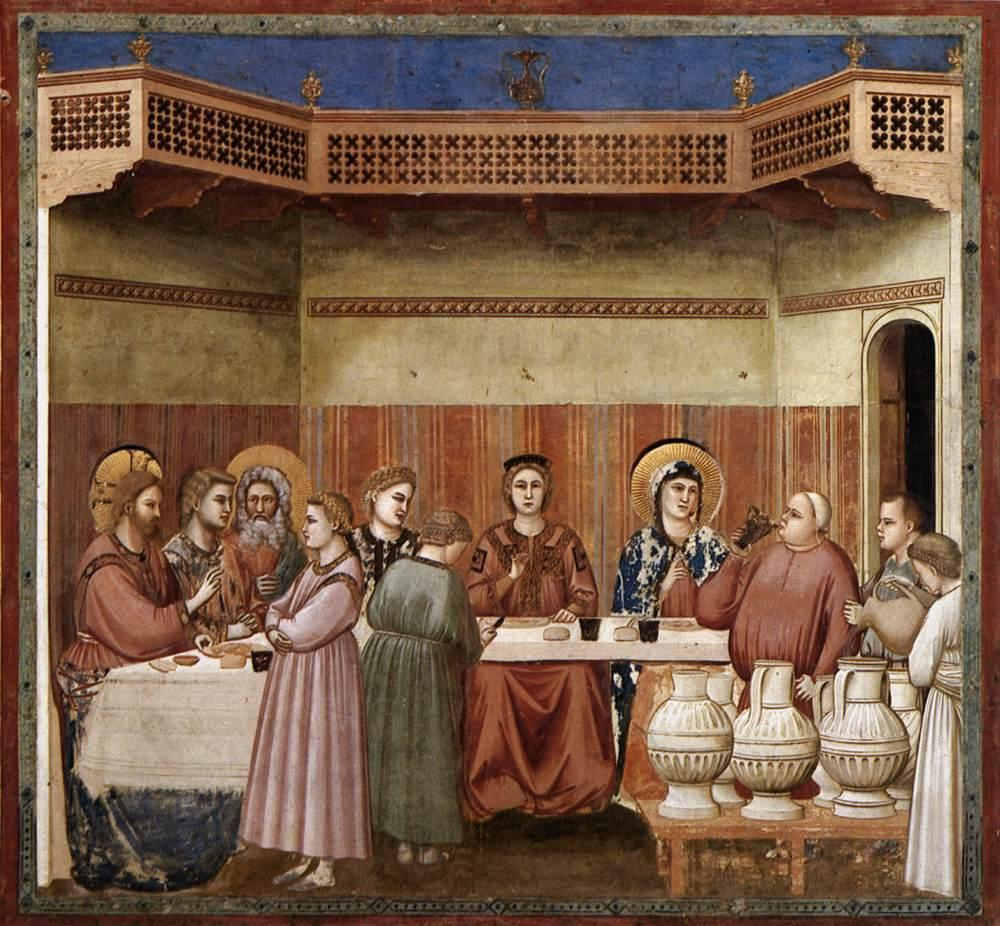
\includegraphics[scale=0.17, trim=0mm 0mm 0mm 0mm, clip=true]{giotto-scrovegni.jpg}
\end{SCfigure}

\clearpage

\section*{\textcolor{forestgreen(traditional)}{\textcalligra{\huge{Chiesa di Camaldola}}}} 
L’appellativo \textit{Camaldola} trova origine nella congregazione monastico-cattolica camaldolese, istituita ad Arezzo tra il 1024 e il 1025 dal monaco benedettino San Romualdo di Ravenna (tra il 951 e il 953-1027). Particolarità di tale congregazione è la coniugazione della dimensione comunitaria con quella solitaria, espresse architettonicamente dalla presenza dell’eremo e del monastero nella stessa struttura. In due secoli la sua fama si espande a tal punto da suscitare il desiderio che anche a Verona si fondi un monastero camaldolese. Lo studio di alcuni documenti attendibili ha permesso di affermare che, grazie a una donazione, nell’ottobre del 1202 inizi l’edificazione di una chiesa ad Avesa, chiamata prima \textit{Santa Maria di Avesa} e in seguito \textit{Il Camaldolino}. Otto anni dopo, a Camaldola si riscontra un monastero doppio, ossia di monaci e converse, e dipendente dall’eremo di Camaldoli aretino. L’analisi delle fonti farebbe risalire al 1598 la fine del monastero, del quale oggi rimane come unica testimonianza la piccola chiesa.\\

Nonostante le numerose manomissioni subite nei secoli (i primi restauri risalirebbero al 1305), la chiesa di Camaldola ha mantenuto un’impronta stilistica romanico-gotica ed è dominata dalla semplicità. La facciata con tetto a capanna, originariamente a mattoni a vista e in pietra tenera locale, presenta un portale cinquecentesco, sormontato da una monofora e da un bassorilievo con l’Agnello Mistico, simbolo di Cristo. L’interno, a pianta rettangolare e tetto a capriate con travature scoperte, è stato sottoposto agli ultimi lavori di restauro negli anni 1987-88. L’affresco sulla parete di destra raffigura una \textit{Maestà}, cioè la Madonna seduta in trono con Gesù bambino. Alla loro destra vi è un santo difficilmente identificabile, al quale ne era probabilmente contrapposto un altro, poi fatto scomparire con l’apertura dell’attuale finestra oblunga. In basso a sinistra si osserva un uomo inginocchiato, senza dubbio il committente della pittura. Alcuni dettagli, come la forma gotica del trono della Vergine e i due angioletti sugli angoli dello stesso hanno suggerito una datazione al XIV secolo.\\ 

\vspace*{-1mm}L’altare, inizialmente addossato all’abside ma smontato e ricomposto nel XVI secolo, appare come un assemblaggio di diversi pezzi e sarebbe ascrivibile alla prima metà del XIV secolo, ovvero al periodo di massima floridezza del monastero avesano. Questo fatto giustificherebbe quindi la finezza e la qualità di esecuzione di alcuni elementi. Il frontale dell’altare è un bassorilievo in pietra della locale Val Gallina sormontato da una cimasa di foglie lussureggianti. Esso è diviso da quattro colonnine, due lisce e due tortili, che delimitano tre scomparti, con arco a tutto sesto al centro e arcatelle ogivali ai lati.  Nella parte centrale siedono su un trono Cristo e la Vergine che, con le braccia incrociate sul petto, si china leggermente verso il figlio per essere incoronata. A destra, un santo vescovo identificato come San Zeno regge un libro nella mano sinistra, mentre la mano destra, che in origine impugnava un pastorale, appare socchiusa. A sinistra, San Romualdo tiene la \textit{Regola} di San Benedetto nella mano sinistra e ha la destra priva del pastorale che un tempo stringeva. I tondi inscritti nei pennacchi recano i simboli zoomorfi dei quattro evangelisti: da sinistra a destra si notano un bue alato (San Luca), un’aquila (San Giovanni), un leone alato (San Marco) e un angelo (San Matteo). Il gradino della mensa è caratterizzato da cinque edicole cuspidate, un tempo policrome e con alcune parti dorate. Si osservano all’estremità sinistra l’arcangelo Gabriele e all’estremità destra la Vergine seduta; ai lati dell’edicola centrale, posta sopra il tabernacolo e raffigurante un \textit{Ecce Homo}, ve ne sono due di minori dimensioni con due santi monaci camaldolesi. Il tabernacolo, trilobo e a ornati floreali, è stato collocato nella posizione attuale intorno al 1957, mentre in precedenza era inserito nella nicchia a destra dell’altare. Esso presenta l’iscrizione a caratteri gotici “\textsc{Mesere don Gironimo a fato faro qu[e]sto lavorero}”, che ha permesso agli studiosi di datare il manufatto alla prima metà del XV secolo. Gli altari laterali sono sormontati da due pale: a destra è posta una \textit{Natività di Maria} di Marcantonio Bassetti (1589-1630), mentre a sinistra, recentemente restaurato, vi è un \textit{San Girolamo}, attribuito a Felice Brusasorzi (1539-1605). 
\clearpage

\section*{\textcolor{forestgreen(traditional)}{\textcalligra{\huge{Camaldola Church}}}} 
\textit{Camaldola} derives its name from a catholic monastic congregation called \textit{Camaldolese}, founded between 1024 and 1025 by the Italian monk Saint Romuald (ca. 951-1027) in Camaldoli, near the city of Arezzo, in central Italy. Camaldolese spirit aims at integrating the hermitic and social dimensions of monastic life, and this is architecturally expressed by the presence of both the hermitage and the monastery in the same structure. Two centuries after its constitution, the celebrity gained by the Camaldolese encouraged the establishment of a new monastery in Verona. Researches across valid historical sources show that, following a donation, in October 1202 a church dedicated to the Virgin Mary begins to be built in the village of Avesa. Eight years later, in Camaldola appeared a double monastery hosting both monks and nuns, which depended on Arezzo’s congregation. Further studies attribute the decline of the monastery in Avesa to the year 1598.\\

Despite the repeated tampering (the first dating back to 1305), Camaldola Church has maintained some Romanesque and Gothic marks, and is characterised by simplicity. The façade was initially in exposed brickwork and local stone; it is decorated with a \nth{16} century portal, on top of which are a single-lancet window and a low relief showing the Mystic Lamb, symbol of Christ. The interior, a rectangular plan with an A-frame roof in plain view, has been lastly restored in 1988-89. The fresco on the right depicts a \textit{Maestà}, i.e. the enthroned Madonna with the child Jesus. At their right hand side stands an unknown saint, who was most likely coupled with a second one, now replaced by the oblong window. At the bottom left is a kneeling man, who is undoubtedly the commissioner of the painting. Some details, such as the Gothic shape on the Madonna’s throne and the angels at its corners, may suggest a dating of the fresco back to the \nth{14} century.\\ 

\vspace*{-1mm}The altar, which was initially leaning against the apse, was dismantled and reassembled in the \nth{16} century. It is a combination of different pieces and has been dated back to the first half of the \nth{14} century, the most flourishing period of the monastery. This could therefore explain the elegance and quality of some of its elements. The front of the altar, a low relief made of local tender stone, is topped with a cymatium of luxuriant leaves. Below this, two straight and two helical columns define three compartments, with a round arch in the middle, and cusped arches at the sides. On the throne of the central unit are seated Christ and the Virgin Mary, who bows down with her arms crossed on her chest to receive the crown. On the right, a man identified with Saint Zeno holds a book in his right hand, while the left was once grasping a crosier. On the opposite side, Saint Romuald holds the \textit{Rule} of Saint Benedict on his right hand, whereas his left hand, originally with a crosier as well, is now empty. The \textit{tondi} inscribed in the pendentives illustrate the zoomorphic symbols of the evangelists: from the far left are a winged ox (Saint Luke), an eagle (Saint John), a winged lion (Saint Marc) and an angel (Saint Matthew). Above the altar are five \textit{aediculae} with pinnacles, which were formerly polychrome and partially gold-plated. On the left knees the archangel Gabriel, while at the right is represented a seated Madonna. The central \textit{aedicula}, placed over the tabernacle, depicts an \textit{Ecce Homo} and is flanked by two smaller ones with two Camaldolese monks. The tabernacle, with a three-foiled cusped arch and a floral motif, was in the niche on the right of the altar before being placed in its current position. At its bottom, an inscription allowed researchers to date it to the first half of the \nth{15} century. This  reads: “\textsc{Mesere don Gironimo a fato faro qu[e]sto lavorero}”, meaning “Father Jerome commissioned this work”. The side altars are decorated with two altarpieces: on the right is suspended a \textit{Nativity of the Virgin} by Marcantonio Bassetti (1589-1630), and on the left a \textit{Saint Jerome} attributed to Felice Brusasorzi (1539-1605) and recently restored.
\clearpage

\thispagestyle{empty}
\begin{flushleft} 
\section*{\textcolor{forestgreen(traditional)}{\textcalligra{\huge{Grazie di cuore\hspace*{1mm}...}}}} 

\noindent … a tutti i familiari e gli amici che sono venuti da vicino e da lontano per festeggiare con noi: i vostri sorrisi e la vostra allegria rendono ancora più grande la nostra gioia in questo momento indimenticabile.\\
\vspace*{3mm}
\noindent Un grazie speciale alle nostre famiglie per averci trasmesso il valore dell’amore e per averci sostenuto in ogni istante nella preparazione di questo giorno.
\end{flushleft}
\vfill
%\begin{center}
%\huge{$\sim \centerdot \backsim$}
%\end{center} 
%\vfill 
\begin{flushright}
\section*{\textcolor{forestgreen(traditional)}{\textcalligra{\huge{Our sincere thanks\hspace*{1mm}...}}}} 

\noindent … to all our relatives and friends gathered here from near and far to celebrate with us: your smiles and cheerfulness enhance our joy in this unforgettable moment.\\
\vspace*{3mm}
A very special thank you to both our families who taught us what love means and have relentlessly supported us during the preparation of this day.
\afterpage{\blankpage}
\end{flushright}

\end{document}